\RequirePackage{shellesc}
\immediate\write18{tex spath3_code.dtx}
\documentclass{l3doc}
\usepackage{tikz}
\usetikzlibrary{
  spath3,
  hobby,
  patterns,
  intersections,
  arrows.meta,
}
 
\usepackage{listings}
\lstloadlanguages{[LaTeX]TeX}
\lstset{
  breakatwhitespace=true,
  breaklines=true,
  language=[LaTeX]TeX,
  basicstyle=\small\ttfamily,
  keepspaces=true,
  columns=fullflexible
}
 
\usepackage{fancyvrb}

\newenvironment{example}
{\VerbatimEnvironment
\begin{VerbatimOut}[gobble=0]{example.out}}
{\end{VerbatimOut}
   \begin{center}
   \setlength{\parindent}{0pt}
   \fbox{\begin{minipage}{.9\linewidth}
     \lstinputlisting[]{example.out}
   \end{minipage}}

   \fbox{\begin{minipage}{.9\linewidth}
     \centering
     \input{example.out}
   \end{minipage}}
\end{center}
}

\providecommand*{\url}{\texttt}
\GetFileInfo{spath3.sty}

\title{The \textsf{spath3} Package: Documentation}
\author{Andrew Stacey \\ \url{loopspace@mathforge.org}}
  \date{\fileversion~from \filedate}

  \begin{document}

  \maketitle

  \section{Introduction}

  The \texttt{spath3} package was originally designed as a low-level package for manipulating the \emph{soft paths} defined by PGF/TikZ.
  Soft paths form one stage of the stack of translations between what the author writes in the \texttt{tikzpicture} environments in their \LaTeX\ document and what is eventually written to the output file.
  Most of the complicated processing has been done by the time a soft path is constructed, but it is still very definitely a \TeX\ object and there has not, for example, been any consideration as to what the eventual output file format is (such as PDF, DVI, or SVG).
  So it is very amenable to being modified at this stage and this package provides a set of routines for doing so.

  The original purpose was to provide a common core on which other packages would be built.
  Indeed, the packages \texttt{calligraphy}, \texttt{knots}, and \texttt{penrose} all use this package.
  However, over time I've found myself wanting to use the routines of this package at a higher level and so have designed some user-level interfaces.
  This document documents those.

  To clarify some terminology, paths are composed of \emph{segment} and \emph{components}.
A \emph{segment} is a minimal drawing piece.
Thus it might be a straight line or a B\'ezier curve.
A \emph{component} is a minimal connected section of the path.
So every component starts with a move command and continues until the next move command.
For ease of implementation (and to enable a copperplate pen in the calligraphy package!), an isolated move is considered as a component.

  
  \section{TikZ Keys}

\begin{lstlisting}
\usetikzlibrary{spath3}
\end{lstlisting}

The \texttt{spath3} TikZ library defines a set of keys that can be issued to muck about with soft paths.
These are all defined in the \texttt{spath} family, so all the following keys should be prefixed by \texttt{spath/}, or the key \texttt{spath/.cd} needs to be used beforehand.

\subsection{Saving and Using Soft Paths}

\begin{function}{save}
\begin{syntax}
|save=|\meta{name}
\end{syntax}

Saves the current path with name \texttt{<name>}.
This delays until the path is fully constructed so can be issued in the options to the main command.

Soft paths constructed this way are local to the group in which the path command is issued.

The soft path is actually stored in a macro constructed from the name.
There are a couple of reasons for using a \emph{name} rather than a macro directly.
One is so that it is compatible with the \texttt{intersections} library -- by default both this package and that save their paths in the same underlying macro.
The other is to provide a way to link a soft path with a set of TikZ styles (this is particularly useful when splitting the path into components).
\end{function}

\begin{function}{save global}
\begin{syntax}
|save global=|\meta{name}
\end{syntax}

Saves the current soft path globally.
\end{function}

\begin{function}{clone}
\begin{syntax}
|clone=|\marg{target}\marg{source}
\end{syntax}

Clones one soft path into another.
\end{function}

\begin{function}{restore}
\begin{syntax}
|restore=|\meta{name}
\end{syntax}

Restores a previously saved soft path to the current path.
This happens immediately so can be issued in the options to the main command and then the path can be extended with normal drawing commands.
Any keys that affect the soft path directly should be applied \emph{before} this one.

One thing should be noted about transformations.
By the time a soft path is built, all available transformations have been applied.
This means that when re-inserting a soft path back into a high level command (such as |\draw|), the effect of existing transformations might produce some confusing effects.
When restoring a path then the library tries to set the last point correctly, but depending on how this is used it can result in transformations being applied twice.
\end{function}

\begin{function}{append}
\begin{syntax}
|append=|\meta{name}
\end{syntax}

This inserts a soft path into the path at the current point, it is therefore more suited to being used part way through a path construction.
In a sense, it is a little like a \texttt{pic} in that it enables the user to construct a path segment early to be reused at various places.

The path is \emph{welded} on to the current path, meaning that it starts from the current point and there is no \texttt{move}.
This is particularly useful for creating filled regions.
\end{function}

\begin{function}{reverse}
\begin{syntax}
|reverse=|\meta{name}
\end{syntax}

Reverses the path in the named spath object.
This doesn't do any actually drawing.
The effect is local, but if you want to work with both the original path and its reversal in the same path then use the \texttt{clone} key to copy it first.
\end{function}

\begin{function}{append reverse}
\begin{syntax}
|append reverse=|\meta{name}
\end{syntax}

Like \texttt{append} except that the inserted path is reversed first.
\end{function}

\begin{function}{insert}
\begin{syntax}
|insert=|\meta{name}
\end{syntax}

Like \texttt{append} except that it doesn't move the inserted path and there is a move between the current path and the inserted path.
\end{function}

\begin{function}{
  shorten at end,
shorten at start,
shorten at both ends
}
\begin{syntax}
|shorten at end=|\marg{name}\marg{dimen}
\end{syntax}

Shortens the soft path by the dimension from one or both ends.
This shortens the soft path along its length so that it is guaranteed that the shorter path traces a subset of the original path.
For B\'ezier curves, however, the amount of shortening is approximate and is better for shorter distances.
If wanting to shorten by a large amount it is better to shorten by a small amount a number of times.
\end{function}

\begin{function}{translate}
\begin{syntax}
|translate=|\marg{name}\marg{x-dimen}\marg{y-dimen}
\end{syntax}

Translates the soft path by the given dimensions.
\end{function}

\begin{function}{transform}
\begin{syntax}
|transform=|\marg{name}\marg{transformations}
\end{syntax}

This applies the transformation to the soft path.
The transformation is processed by TikZ so should consist of TikZ-level transformations such as |shift={(2,2)}|.
\end{function}

\subsection{Intersection Routines}

To use these features you need to use the \texttt{intersections} library.

\begin{function}{split at self intersections}
\begin{syntax}
|split at self intersections=|\meta{path}
\end{syntax}

This inserts breaks into the named soft path at the points where it intersects itself.
\end{function}

\begin{function}{split at intersections}
\begin{syntax}
|split at intersections=|\marg{first}\marg{second}
\end{syntax}

This inserts breaks into a pair of paths at their mutual intersections.
\end{function}

\subsection{Working with Components}

\begin{function}{get components of}
\begin{syntax}
|get components of=|\marg{macro}\marg{path}
\end{syntax}
  
This splits the path into a list of its components, which are stored in the macro.
The macro can be used in a |\foreach|.
\end{function}

\begin{function}{render components}
\begin{syntax}
|render components=|\meta{path}
\end{syntax}

This renders the components of a given path as separate TikZ commands, so that each can be separately styled.
It applies the following styles (in this order):

\begin{enumerate}
\item \texttt{every spath component}
\item \texttt{spath component <number>}
\item \texttt{spath component=<number>}
\item \texttt{every <path> component}
\item \texttt{<path> component <number>}
\item \texttt{<path> component=<number>}
\end{enumerate}
\end{function}

\begin{function}{insert gaps after components}
\begin{syntax}
|insert gaps after components=|\marg{path}\marg{gap}\marg{components}
\end{syntax}

This inserts a gap between components of a path by shortening the end of the specified component and start of the next one.
The list of components is passed through a |\foreach| loop so that syntax like |2,4,...,16|.
\end{function}

\begin{function}{join components}
\begin{syntax}
|join components=|\marg{path}\marg{components}
\end{syntax}

This removes the \texttt{move} between the given component and the previous one.
If the component is the first one then it is joined to the last component.
\end{function}

\begin{function}{spot weld}
\begin{syntax}
|spot weld=|\meta{path}
\end{syntax}

This removes the \texttt{move} between any two components of the path where the end point of one component is the same as the initial point of the next (the tolerance on error here is \(0.01\)pt).
\end{function}

\begin{function}{remove empty components}
\begin{syntax}
|remove empty components=|\meta{path}
\end{syntax}

This removes empty components of the path (which consist of simply a move).
\end{function}

\subsection{Shortening Paths}

\begin{function}{
shorten path at end,
shorten path at start,
shorten path at both ends
}
\begin{syntax}
|shorten path at end=|\marg{path}\marg{length}
\end{syntax}

This shortens a path by the given amount from the specified end.
The shortening is done so that it guarantees that it lies along the original path, but therefore the length is not completely guaranteed to be accurate.
This is particularly true for B\'ezier paths and if there is a very short segment at the end.

It uses the derivative at the end to work out how much to shorten by.
\end{function}

\subsection{Exporting Paths}

There are two keys to export a path.

\begin{function}{save to aux}
\begin{syntax}
|save to aux=|\meta{path}
\end{syntax}

This will save the path to the auxfile so that it is available again on the next run through.
\end{function}

\begin{function}{export to svg}
\begin{syntax}
|export to svg=|\meta{path}
\end{syntax}

Saves the path to the file \texttt{path.svg} as an SVG document.
\end{function}

\subsection{Knots}

\begin{function}{knot}
\begin{syntax}
|knot=|\meta{path}\meta{gap}\meta{components}
\end{syntax}

This style combines various of the above to make it simpler to draw knots and links.
It expands to:

\begin{lstlisting}
knot/.style n args={3}{
  spath/.cd,
  split at self intersections=#1,
  insert gaps after components={#1}{#2}{#3},
  maybe spot weld=#1,
  render components=#1
}
\end{lstlisting}

This splits a path at the points where it self-intersects and then inserts gaps between specified components.
The key |maybe spot weld| does a |spot weld| depending on whether or not the key |draft mode| is set to |true| or |false|.
The point here is that when designing the knot it is useful to not weld together components since that changes the component count.
But once the gaps are inserted in the desired places, welding the remaining components produces a nicer diagram.

The components can be styled using the keys as described in |render components|.
\end{function}

\subsection{Coordinates}

Soft paths are not natural TikZ objects and so when replaced back into a TikZ path construction then they don't fully interact with other TikZ things, like placing nodes at points on the path.
To make things a little easier there is defined a coordinate system which identifies a point at a certain location along a soft path.

The location specification is a little technical.
It is specified as a number from \(0\) to \(1\), but the parameter works as follows.
Let \(n\) be the number of \emph{segments} on the path (these are the individual drawing elements that make up the path).
The interval from \(\frac{k-1}{n}\) to \(\frac{k}{n}\) is assigned to the \(k\)th segment of the path.
Then for a parameter in that interval, the location uses the natural parametrisation of that segment.
For a straight line, it is simply the proportional position along but for a B\'ezier curve then it uses the B\'ezier parametrisation.

The syntax for this is:
%
\begin{lstlisting}
(spath cs:<name> <parameter>)
\end{lstlisting}
%
The space is vital, so if the \texttt{name} is contained in a macro then a space has to be inserted somehow.
One option is to wrap the macro in braces, as seen in the examples in the next section.

\section{Examples}

\begin{enumerate}
\item Saving, restoring, inserting, and appending.

\begin{example}
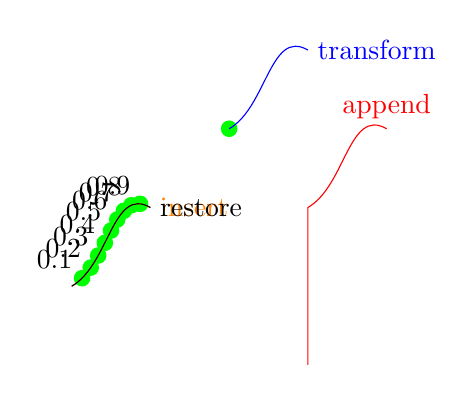
\begin{tikzpicture}
\path[spath/save=rpath] (0,0) to[out=30,in=150] (1,1);
\foreach \k in {1,...,9} {
  \fill[green] (spath cs:rpath 0.\k) circle[radius=3pt];
  \node[above left] at (spath cs:rpath 0.\k) {\(0.\k\)};
}
\fill[green] (2,2) circle[radius=3pt];
\draw[blue, spath/transform={rpath}{shift={(2,2)}}, spath/restore=rpath] node[right] {transform};
\draw[orange] (3,0) [spath/insert=rpath] node[right] {insert};
\draw[red] (3,-1) -- +(0,2) [spath/append=rpath] node[above] {append};
\draw[spath/restore=rpath] node[right] {restore};
\end{tikzpicture}
\end{example}

\item Reversing.

\begin{example}
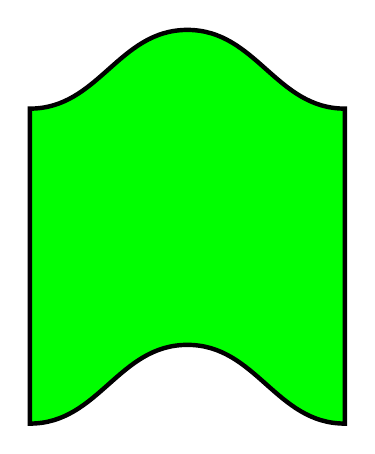
\begin{tikzpicture}
\path[spath/save=apath] (0,0) to[out=0,in=180] (2,1) to[out=0,in=180] (4,0);
\filldraw[
  green,
  draw=black,
  ultra thick,
  spath/restore=apath
] -- ++(0,-4) [spath/append reverse=apath] -- cycle;
\end{tikzpicture}
\end{example}

\item Transformations.

\begin{example}
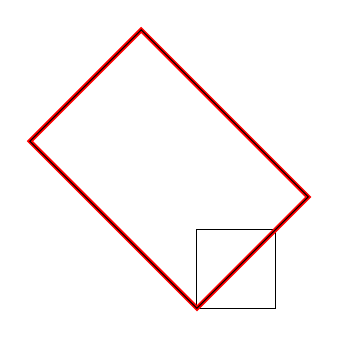
\begin{tikzpicture}
\draw[spath/save=tpath] (0,0) rectangle +(1,1);
\draw[rotate=45, xscale=2, yscale=3, ultra thick, red] (0,0) rectangle +(1,1);
\draw[
  spath/transform={tpath}{rotate=45, xscale=2, yscale=3},
  spath/restore={tpath}];
\end{tikzpicture}
\end{example}

\item Shortening.

\begin{example}
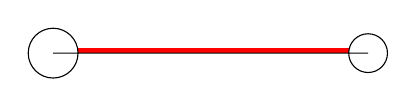
\begin{tikzpicture}
\path[spath/save=apath] (0,0) foreach \k in {1,...,4} { -- ++(1,0) +(0,0)};
\draw[
  spath/shorten at end={apath}{7pt},
  spath/shorten at start={apath}{9pt},
  spath/translate={apath}{0pt}{1pt},
  spath/restore=apath,
  ultra thick, red
];
\draw (0,0) circle[radius=9pt] [spath/insert=apath] circle[radius=7pt];
\end{tikzpicture}
\end{example}


\begin{example}
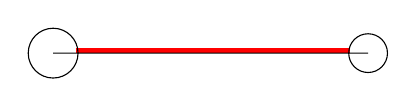
\begin{tikzpicture}
\path[spath/save=apath] (0,0) foreach \k in {1,...,4} { to[out=0,in=180] ++(1,0) +(0,0)};
\draw[
  ultra thick,
  red,
  spath/.cd,
  shorten at end={apath}{7pt},
  shorten at start={apath}{9pt},
  translate={apath}{0pt}{1pt},
  restore=apath,
];
\draw (0,0) circle[radius=9pt] [spath/insert=apath] circle[radius=7pt];
\end{tikzpicture}
\end{example}

\begin{example}
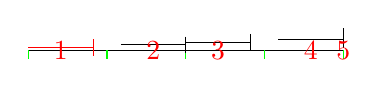
\begin{tikzpicture}
\draw[spath/save=npath] (0,0) foreach \k in {1,...,4} { -- ++(1,0) +(0,0)};
\draw[green] (0,0) -- +(0,-3pt) foreach \k in {1,...,4} { -- +(0,-3pt) ++(1,0)} -- +(0,-3pt);

\tikzset{
  spath/.cd,
  insert gaps after components={npath}{10pt}{1,3},
  get components of={npath}\components,
}

\tikzset{
  path 1/.style={
    red,
  },
}

\foreach[count=\k] \cpt in \components {
  \path[
    draw,
    path \k/.try,
    spath/.cd,
    translate=\cpt{0pt}{\k pt},
    restore=\cpt,
  ] +(0,3pt) -- +(0,-3pt);
  \node[text=red] at (spath cs:{\cpt} .5) {\(\k\)};
}
\end{tikzpicture}
\end{example}

\item Intersections.

One of the main motivations for implementing the intersection routines was to provide a different way of drawing knots and links and similar diagrams.

\begin{enumerate}

\item Define the two paths for the braid (usually these will be defined with |\path|).
\begin{example}
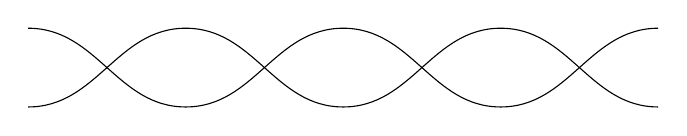
\begin{tikzpicture}[
  use Hobby shortcut,
]
\draw[spath/save global=pathA] (0,0) to[out=0,in=180] ++(2,1) to[out=0,in=180] ++(2,-1)  to[out=0,in=180] ++(2,1)  to[out=0,in=180] ++(2,-1);
\draw[spath/save global=pathB] (0,1) to[out=0,in=180] ++(2,-1) to[out=0,in=180] ++(2,1)  to[out=0,in=180] ++(2,-1)  to[out=0,in=180] ++(2,1);
\end{tikzpicture}
\end{example}

\item Split the paths at their mutual intersections and render them with a count of the components.

\begin{example}
\begin{tikzpicture}
\tikzset{
  spath/.cd,
  split at intersections={pathA}{pathB},
  get components of={pathA}\pathAcomponents,
  get components of={pathB}\pathBcomponents,
}

\foreach[count=\k] \cpt in \pathAcomponents {
  \draw[spath/restore=\cpt,-Circle];
  \node[fill=white, fill opacity=.5, circle, text opacity=1] at (spath cs:{\cpt} .5) {\(\k\)};
}

\foreach[count=\k] \cpt in \pathBcomponents {
  \draw[spath/restore=\cpt,-Circle];
  \node[fill=white, fill opacity=.5, circle, text opacity=1] at (spath cs:{\cpt} .5) {\(\k\)};
}
\end{tikzpicture}
\end{example}

\item Now we insert gaps after certain components in each path and then render the components.
To show that the gaps are genuine, we use a patterned background.
Although the paths were defined globally, the splitting in the previous example was local so we need to repeat it in this one.

\begin{example}
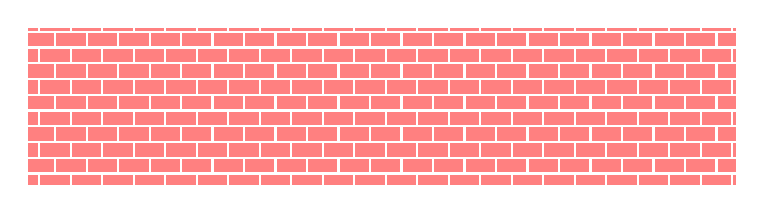
\begin{tikzpicture}
\tikzset{
  spath/.cd,
  split at intersections={pathA}{pathB},
  insert gaps after components={pathA}{5pt}{1,3},
  join components={pathA}{3,5},
  get components of={pathA}\pathAcomponents,
  insert gaps after components={pathB}{5pt}{2,4},
  join components={pathB}{2,4},
  get components of={pathB}\pathBcomponents,
}

\fill[red!50!white] (-.5,-.5) rectangle (8.5,1.5);
\fill[pattern=bricks, pattern color=white] (-.5,-.5) rectangle (8.5,1.5);

\foreach[count=\k] \cpt in \pathAcomponents {
  \draw[blue, line width=2pt,spath/restore=\cpt];
  \node[fill=cyan, fill opacity=.5, circle, text opacity=1] at (spath cs:{\cpt} .3) {\(\k\)};
}

\foreach[count=\k] \cpt in \pathBcomponents {
  \draw[green, line width=2pt,spath/restore=\cpt];
  \node[fill=green!50, fill opacity=.5, circle, text opacity=1] at (spath cs:{\cpt} .3) {\(\k\)};
}
\end{tikzpicture}
\end{example}
\end{enumerate}

\item This example is notable because many of the intersection points are where segments of the path end, showing that the algorithm works well even in this circumstance.

\begin{enumerate}
\item Here's the original path.
\begin{example}
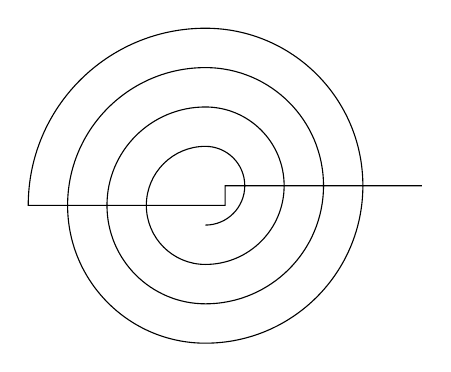
\begin{tikzpicture}
\draw[spath/save global=spiral] (5,0) -- (2.5,0) -- ++(0,-.25) -- ++(-2.5,0)
arc[radius=2.25cm,start angle=180,end angle=90]
arc[radius=2cm,start angle=90, delta angle=-180]
arc[radius=1.75cm,start angle=-90, delta angle=-180]
arc[radius=1.5cm,start angle=90, delta angle=-180]
arc[radius=1.25cm,start angle=-90, delta angle=-180]
arc[radius=1cm,start angle=90, delta angle=-180]
arc[radius=.75cm,start angle=-90, delta angle=-180]
arc[radius=.5cm,start angle=90, delta angle=-180]
;
\end{tikzpicture}
\end{example}

\item This renders labels on each component after splitting.
\begin{example}
\begin{tikzpicture}
\tikzset{
  spath/.cd,
  split at self intersections=spiral,
  get components of={spiral}\pathcomponents,
}

\foreach[count=\k] \cpt in \pathcomponents {
  \draw[spath/restore=\cpt,-|];
  \node[fill=white, fill opacity=.5, circle, text opacity=1] at (spath cs:{\cpt} .5) {\(\k\)};
}
\end{tikzpicture}
\end{example}

\item Finally, we put the gaps in where we want them.

\begin{example}
\begin{tikzpicture}
\tikzset{
  spath/.cd,
  split at self intersections=spiral,
  insert gaps after components={spiral}{10pt}{1,3,5,7,10,11,14},
  spot weld=spiral,
  get components of={spiral}\pathcomponents,
}

\foreach[count=\k] \cpt in \pathcomponents {
  \draw[blue, line width=2pt,spath/restore=\cpt];
}
\end{tikzpicture}
\end{example}
\end{enumerate}

\item Here's a trefoil knot, demonstrating the \texttt{knot} style that simplifies creating knots.
\begin{example}
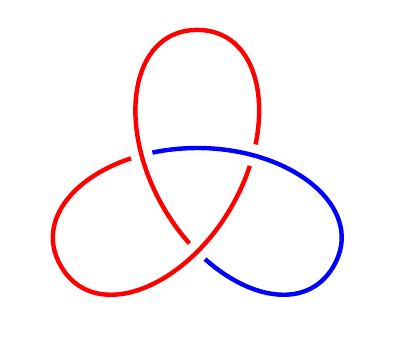
\begin{tikzpicture}[
  use Hobby shortcut,
  every trefoil component/.style={ultra thick, draw, red},
  trefoil component 1/.style={blue},
]
\path[spath/save=trefoil] ([closed]90:2) foreach \k in {1,...,3} { .. (-30+\k*240:.5) .. (90+\k*240:2) } (90:2);
\tikzset{spath/knot={trefoil}{8pt}{1,3,5}}
\end{tikzpicture}
\end{example}
\end{enumerate}
  \end{document}
